%----------------------------------------------------------------------------------------
%    PACKAGES AND THEMES
%----------------------------------------------------------------------------------------

\documentclass[aspectratio=169,xcolor=dvipsnames]{beamer}
\usetheme{SimpleDarkBlue}

\usepackage{hyperref}
\usepackage{graphicx} % Allows including images
\usepackage{booktabs} % Allows the use of \toprule, \midrule and \bottomrule in tables

%----------------------------------------------------------------------------------------
%    TITLE PAGE
%----------------------------------------------------------------------------------------

\title{Hamiltonian Simulation}
\subtitle{Quantum Computing}

\author{Álvaro Sánchez-Paniagua, Ana Vargas, Gonzalo, Íñigo, Miguel Laredo}

\institute
{
    Based on the notes from Ashley Montaro % Your institution for the title page
}
\date{\today} % Date, can be changed to a custom date

%----------------------------------------------------------------------------------------
%    PRESENTATION SLIDES
%----------------------------------------------------------------------------------------

\begin{document}

\begin{frame}
    % Print the title page as the first slide
    \titlepage
\end{frame}

\begin{frame}{Motivation}
\end{frame}


\begin{frame}{Overview}
    % Throughout your presentation, if you choose to use \section{} and \subsection{} commands, these will automatically be printed on this slide as an overview of your presentation
    \tableofcontents
\end{frame}





%%%%%%%%%%%%%%%%%%%
% Ana
%%%%%%%%%%%%%%%%%%%

\section{Introduction}
\begin{frame}{Introduction: Hamiltonian \textcolor{lightgray}{Simulation}}
    \begin{block}{Hamiltonian}
        Hermitian operator acting on $n$ qubits which corresponds physically to a system made up of $n$ 2-level subsystems.
    \end{block}
    \begin{block}{Schrödinger’s equation}
        Time evolution of the state $|\psi\rangle$ of a quantum system:
        \begin{align*}
            i \hbar \frac{d}{dt}|\psi(t)\rangle = H(t)|\psi(t)\rangle
        \end{align*}
    \end{block}
\end{frame}

\begin{frame}{Introduction: \textcolor{lightgray}{Hamiltonian} Simulation}
    Solution of the Schrödinger’s equation (\textit{time-independent}):
    \begin{align*}
        |\psi(t)\rangle = e^{-iHt}|\psi(0)\rangle
    \end{align*}
    \begin{block}{Goal}
        To approximate the unitary operator:
        \begin{align*}
            U(t) =  e^{-iHt}
        \end{align*}
    \end{block}
    Approximation in the operator (spectral) norm:
    \begin{align*}
        ||A|| := \max_{|\psi\rangle \neq 0}\frac{||A|\psi\rangle||}{|||\psi\rangle||}.
    \end{align*}
    $\~{U}$ approximates $U$ within $\epsilon$ if
        \begin{align*}
            ||\~{U} - U|| < \epsilon
        \end{align*}
\end{frame}


%%%%%%%%%%%%%%%%%%%
% Alvaro
%%%%%%%%%%%%%%%%%%%

%%%%%%%%%%%%%%%%%%%
% Miguel
%%%%%%%%%%%%%%%%%%%

\begin{frame}{Proportional Case}
  \begin{block}{Hamiltonian is proportional to Pauli Tensor Product}
    We consider the simple case where $H$ is proportional to a Pauli matrix on $n$ qubits:
    \begin{equation*}
      H = \alpha s_1 \otimes s_2 \otimes \cdots \otimes s_n
    \end{equation*}
  \end{block}
  \begin{block}{Time Evolution Operator (What we are trying to compute)}
    \begin{equation*}
      e^{-i t H} = e^{-i t \alpha s_1 \otimes s_2 \otimes \cdots \otimes s_n}.
    \end{equation*}
  \end{block}
  \begin{block}{Matrix Exponential}
    For any square matrix $A \in \mathbb{C}^{n \times n}$, the matrix exponential is defined by:
    \small{
    \[
      e^A = \sum_{k=0}^{\infty} \frac{A^k}{k!} = I + A + \frac{A^2}{2!} + \frac{A^3}{3!} + \cdots
    \]
    }
  \end{block}
\end{frame}

\begin{frame}{Diagonalizing H}
  \begin{block}{Walkthrough of how to make H diagonal}
    \begin{equation*}
      H = \alpha s_1 \otimes s_2 \otimes \cdots \otimes s_n.
    \end{equation*}
  \end{block}
  \begin{equation*}
    X = \begin{pmatrix} 0 & 1 \\ 1 & 0 \end{pmatrix}, \quad
    Y = \begin{pmatrix} 0 & -i \\ i & 0 \end{pmatrix}, \quad
    Z = \begin{pmatrix} 1 & 0 \\ 0 & -1 \end{pmatrix}
  \end{equation*}

  \begin{itemize}
  \item \textbf{Identity}:
    \begin{equation*}
      I I I^\dagger = I
    \end{equation*}

  \item \textbf{Pauli-Z}:
    \begin{equation*}
      I Z I^\dagger = Z
    \end{equation*}
  \item \textbf{Pauli-X}:
    \begin{equation*}
      HXH^{\dagger} = Z
    \end{equation*}

  \item \textbf{Pauli-Y}:
    \begin{equation*}
      U_Y Y U_Y^\dagger = Z \quad \text{where} \quad U_Y = \frac{1}{\sqrt{2}}\begin{pmatrix} 1 & 1 \\ i & -i \end{pmatrix}
    \end{equation*}

  \end{itemize}

  
\end{frame}




\begin{frame}{Diagonalization of H}
\begin{lemma}[Product of Diagonal Matrices]
Let $D = \mathrm{diag}(d_1,\ldots,d_n)$ and $E = \mathrm{diag}(e_1,\ldots,e_n)$ be diagonal matrices. Then their matrix product is diagonal:
\[
DE = \mathrm{diag}(d_1e_1, \ldots, d_ne_n)
\]
\end{lemma}
\begin{lemma}[Tensor Product of Diagonal Matrices]
Let $A = \mathrm{diag}(a_1,\ldots,a_m)$ and $B = \mathrm{diag}(b_1,\ldots,b_n)$ be diagonal matrices. Then their tensor product is diagonal:
\[
A \otimes B = \mathrm{diag}(a_1b_1, a_1b_2, \ldots, a_mb_{n-1}, a_mb_n)
\]
\end{lemma}

\end{frame}

\begin{frame}{Diagonalization of H}
  \begin{align*}
    H &= \alpha (s_1 \otimes \cdots \otimes s_n) \\
      &= \alpha (U_1 z_1 U_1^\dagger) \otimes \cdots \otimes (U_n z_n U_n^\dagger) \quad \text{(Diagonalize each $s_i$)} \\
      &= \alpha (U_1 \otimes \cdots \otimes U_n)(z_1 \otimes \cdots \otimes z_n)(U_1^\dagger \otimes \cdots \otimes U_n^\dagger)
  \end{align*}
  And thus, 
  \begin{equation*}
    e^{-i t H} = e^{-i \alpha t (U_1 \otimes \cdots \otimes U_n)(z_1 \otimes \cdots \otimes z_n)(U_1^\dagger \otimes \cdots \otimes U_n^\dagger)}
  \end{equation*}

\end{frame}



\begin{frame}

    \begin{equation*}
    e^{-i t H} = e^{-i \alpha t (U_1 \otimes \cdots \otimes U_n)(z_1 \otimes \cdots \otimes z_n)(U_1^\dagger \otimes \cdots \otimes U_n^\dagger)}
  \end{equation*}

  \begin{block}{The conjugation property of the matrix exponential}
    \begin{equation*}
      e^{U H U^{\dagger}} = U e^{H} U^{\dagger}
    \end{equation*}
    This identity is easily proven using the power series definition for matrix exponential. 
  \end{block}

  we diagonalize $e^{-i t H}$ with an appropriate unitary transformation:

  \begin{equation*}
    \begin{align*}
    e^{-i t H} =& e^{-i \alpha t (U_1 \otimes \cdots \otimes U_n)(z_1 \otimes \cdots \otimes z_n)(U_1^\dagger \otimes \cdots \otimes U_n^\dagger)}\\
    =& (U_1 \otimes U_2 \otimes \cdots \otimes U_n) e^{-i \alpha t z_1 \otimes z_2 \otimes \cdots \otimes z_n} (U_1^{\dagger} \otimes U_2^{\dagger} \otimes \cdots \otimes U_n^{\dagger}),
    \end{align*}
  \end{equation*}
  where $z_i \in \{I, Z\}$.
\end{frame}


\begin{frame}{Implementation via Quantum Circuits}
  The main challenge reduces to implementing:
  \begin{equation}
    e^{-i \alpha t Z \otimes Z \otimes \cdots \otimes Z}.
  \end{equation}

  The action of the $k$-qubit $Z$-interaction unitary on a computational basis state is given by:

\[
e^{-i\alpha t Z \otimes \cdots \otimes Z} |x\rangle = 
\begin{cases} 
e^{-i\alpha t} |x\rangle & \text{if } \sum_{i=1}^k x_i \text{ is even} \\
e^{i\alpha t} |x\rangle & \text{if } \sum_{i=1}^k x_i \text{ is odd}
\end{cases}
\]

\end{frame}

\begin{frame}{Quantum Circuit for $k=4$}
  \begin{center}
    \begin{figure}[htbp]
      \centering
      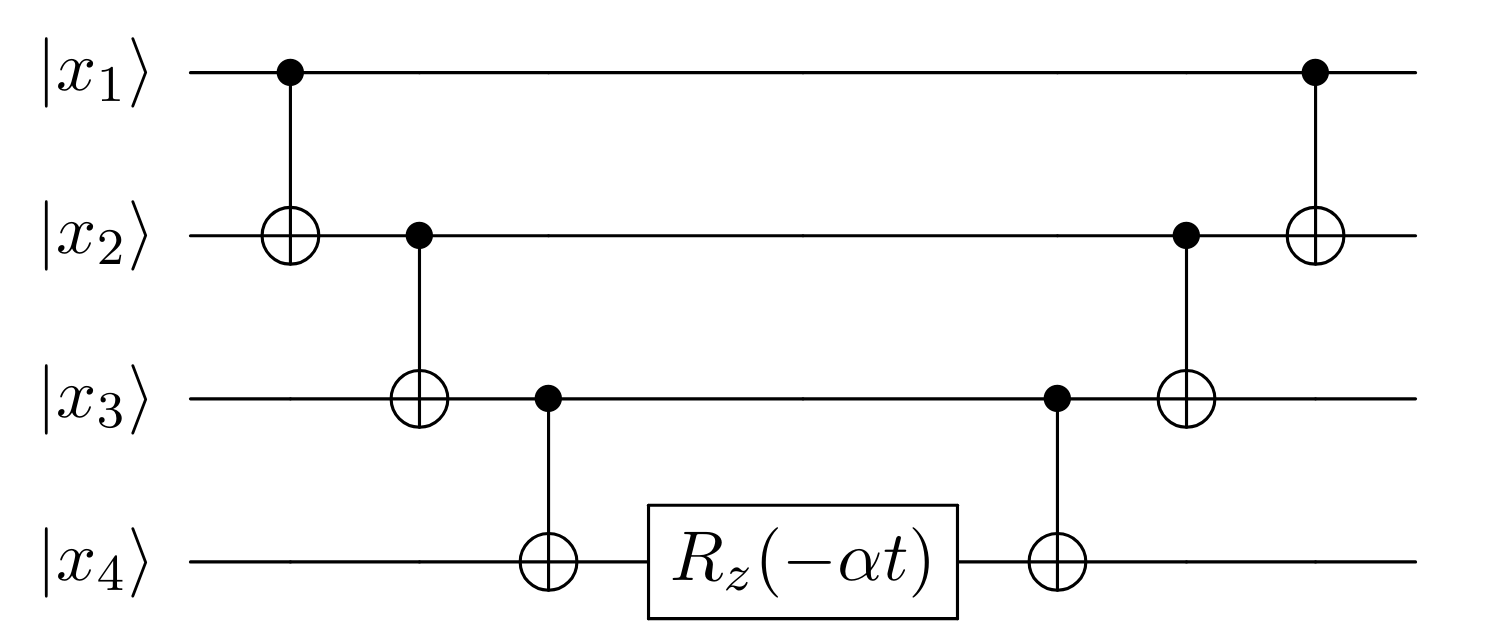
\includegraphics[width=0.8\textwidth]{rsc/circuit.png}
    \end{figure}

  \end{center}
  $R_z(\theta) = \begin{bmatrix} e^{i \theta} & 0 \\ 0 & e^{-i \theta} \end{bmatrix}$
\end{frame}

\begin{frame}{Generalization to Weighted Sums of Pauli Matrices}
  For $H$ as a weighted sum of commuting Pauli matrices:
  \begin{equation}
    H = \sum_{j=1}^{m} \alpha_j \sigma_{s_j},
  \end{equation}
  the evolution follows as:
  \begin{equation}
    e^{-i H t} = \prod_{j=1}^{m} e^{-i \alpha_j \sigma_{s_j} t}.
  \end{equation}
  This requires $O(mn)$ quantum gates.
\end{frame}

%%%%%%%%%%%%%%%%%%%
% Gonzalo
%%%%%%%%%%%%%%%%%%%

%%%%%%%%%%%%%%%%%%%
% Inigo
%%%%%%%%%%%%%%%%%%%


\end{document}
